\begin{figure}[ht]
\centering
% Thesis-wide categorical color palette
% Usage: % Thesis-wide categorical color palette
% Usage: % Thesis-wide categorical color palette
% Usage: \input{figures/palette} in any figure file
%
% Muted primary colors -- print-friendly, visually distinct.
% Inspired by Cooper Union's red/blue primaries, softened for
% academic figures. Use palA-palC for data series in scatter
% plots, line charts, bar charts, etc.

\definecolor{palA}{HTML}{1F77B4}   % Tableau blue
\definecolor{palB}{HTML}{D62728}   % Tableau red
\definecolor{palC}{HTML}{2CA02C}   % Tableau green
 in any figure file
%
% Muted primary colors -- print-friendly, visually distinct.
% Inspired by Cooper Union's red/blue primaries, softened for
% academic figures. Use palA-palC for data series in scatter
% plots, line charts, bar charts, etc.

\definecolor{palA}{HTML}{1F77B4}   % Tableau blue
\definecolor{palB}{HTML}{D62728}   % Tableau red
\definecolor{palC}{HTML}{2CA02C}   % Tableau green
 in any figure file
%
% Muted primary colors -- print-friendly, visually distinct.
% Inspired by Cooper Union's red/blue primaries, softened for
% academic figures. Use palA-palC for data series in scatter
% plots, line charts, bar charts, etc.

\definecolor{palA}{HTML}{1F77B4}   % Tableau blue
\definecolor{palB}{HTML}{D62728}   % Tableau red
\definecolor{palC}{HTML}{2CA02C}   % Tableau green

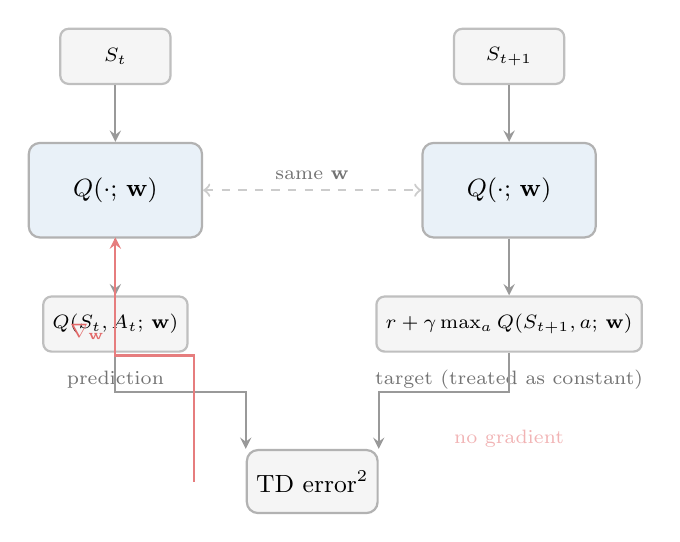
\begin{tikzpicture}[
    net/.style={draw=black!30, thick, rounded corners=4pt,
                minimum width=2.2cm, minimum height=1.2cm,
                font=\small, align=center, inner sep=5pt,
                fill=palA!10},
    io/.style={draw=black!25, thick, rounded corners=3pt,
               minimum width=1.4cm, minimum height=0.7cm,
               font=\scriptsize, fill=black!4, align=center},
    lossbox/.style={draw=black!30, thick, rounded corners=4pt,
                    minimum width=1.4cm, minimum height=0.8cm,
                    font=\small, fill=black!4},
    arr/.style={->, thick, >=stealth, black!40},
    garr/.style={->, thick, >=stealth, palB!60},
    nogarr/.style={thick, palB!25, dashed},
    lbl/.style={font=\scriptsize, text=black!55},
]

% Prediction side (left)
\node[io] (s) at (-2.5, 2.2) {$S_t$};
\node[net] (net1) at (-2.5, 0.5) {$Q(\cdot;\, \mathbf{w})$};
\node[io] (pred) at (-2.5, -1.2)
    {$Q(S_t, A_t;\, \mathbf{w})$};
\node[lbl] at (-2.5, -1.9) {prediction};

\draw[arr] (s) -- (net1);
\draw[arr] (net1) -- (pred);

% Target side (right)
\node[io] (sp) at (2.5, 2.2) {$S_{t+1}$};
\node[net] (net2) at (2.5, 0.5) {$Q(\cdot;\, \mathbf{w})$};
\node[io] (targ) at (2.5, -1.2)
    {$r + \gamma \max_a Q(S_{t+1}, a;\, \mathbf{w})$};
\node[lbl] at (2.5, -1.9) {target (treated as constant)};

\draw[arr] (sp) -- (net2);
\draw[arr] (net2) -- (targ);

% "same w" indicator
\draw[thick, black!20, dashed, <->]
    (net1.east) -- (net2.west)
    node[midway, above, lbl] {same $\mathbf{w}$};

% Loss
\node[lossbox] (loss) at (0, -3.2) {TD error$^2$};
\draw[arr] (pred.south) -- ++(0, -0.5) -| (loss.north west);
\draw[arr] (targ.south) -- ++(0, -0.5) -| (loss.north east);

% Gradient arrow (only to prediction side)
\draw[garr] (-1.5, -3.2) -- (-1.5, -1.6) -- (-2.5, -1.6)
    -- (-2.5, -0.1)
    node[lbl, pos=0.2, left, text=palB!70]
    {$\nabla_{\mathbf{w}}$};

% No gradient on target side (crossed out)
\node[font=\scriptsize, text=palB!35] at (2.5, -2.65)
    {no gradient};

\end{tikzpicture}
\caption{Semi-gradient update. The same parameters $\mathbf{w}$
  produce both the prediction and the target, but the gradient flows
  only through the prediction side.}
\label{fig:semi-gradient}
\end{figure}
